% Use only LaTeX2e, calling the article.cls class and 12-point type.

\documentclass[12pt]{article}
\usepackage{booktabs}
\usepackage{dcolumn}
\usepackage{lscape}
\usepackage[titletoc,title]{appendix}
\usepackage[linkcolor=black,
			colorlinks=true,
			urlcolor=black,
			pdfstartview={XYZ null null 1.00},
			pdfpagemode=UseNone,
			citecolor={black},
			pdftitle={Propagation of Error}]{hyperref}
\usepackage{setspace}		     % Permits line spacing control. Options are \doublespacing, \onehalfspace
\usepackage{longtable}
\usepackage{verbatim}
\usepackage{graphicx}                % Handles inclusion of major graphics formats and allows use of 
\usepackage{fancyhdr}		     % Permits header customization. See header section below.
\usepackage{url}                     % Correctly formats URLs with the \url{} tag
\usepackage{fullpage}		%1-inch margins
\usepackage{multirow}
\usepackage{rotating}
\usepackage{comment}

% Users of the {thebibliography} environment or BibTeX should use the
% scicite.sty package, downloadable from *Science* at
% http://www.sciencemag.org/authors/preparing-manuscripts-using-latex 
% This package should properly format in-text
% reference calls and reference-list numbers.

\usepackage{scicite}
\usepackage{chngcntr}

\usepackage{times}

% The preamble here sets up a lot of new/revised commands and
% environments.  It's annoying, but please do *not* try to strip these
% out into a separate .sty file (which could lead to the loss of some
% information when we convert the file to other formats).  Instead, keep
% them in the preamble of your main LaTeX source file.


% The following parameters seem to provide a reasonable page setup.

\topmargin 0.0cm
\oddsidemargin 0.2cm
\textwidth 16cm 
\textheight 21cm
\footskip 1.0cm


%The next command sets up an environment for the abstract to your paper.

\newenvironment{sciabstract}{%
\begin{quote} \bf}
{\end{quote}}

\begin{comment}

setwd(paste0(githubdir, "propagation_of_error/ms/"))
tools::texi2dvi("error.tex", pdf = TRUE, clean = TRUE) 
setwd(basedir)
  
\end{comment}

\begin{document}
\title{Propagation of Error: Approving Citations to Problematic Research} 

\author
{Ken Cor and Gaurav Sood}

\date{}

% Double-space the manuscript.

\baselineskip24pt

% Make the title.

\maketitle 

\begin{sciabstract}
Reports of serious errors in published research are increasingly common. Once the issues have been made public, we expect \textit{approving} citations to the problematic articles---citations noting no concerns with the cited article---to stop. Using a novel database of over 3,000 retracted articles and nearly 74,000 citations to the retracted articles as well as data from a prominent article that highlights a statistical error in a set of articles published in prominent journals, we estimate citation rates and rates of approving citations pre- and post- notification. We find that at least 31.2\% of the citations to retracted articles happen a year after the article has been retracted. And that 91.4\% of these post-retraction citations are \textit{approving}. We also find that problematic research continues to be approvingly cited long after the problems have been publicized. Our results have implications for the design of scholarship discovery systems and scientific practice more generally.
\end{sciabstract}

\clearpage

Citations are the bedrock of the scientific process. Scientists use citations to give credit for being first (``$x$, $y$, and $z$ have studied $a$''), to debate methods and inferences (``the method used in study $x$ fails to account for $s$''), as evidence (``$x$ shows $a$'', ``we use data from $x$ for our meta-analysis''), and to contextualize results (``our results are consistent with results from $y$''). And unless the researcher notes problems with cited research, citations convey that the results can be trusted.

When researchers \textit{approvingly} cite---cite without noting any concerns---articles with serious errors, problems ensue. First, when such articles (e.g. \cite{rubio2005spontaneous} as noted by \cite{torsvik2010spontaneous}) are approvingly cited as evidence, e.g., \cite{chang2013safety}, it cues that the evidence for the claim is good. Such citations thus unduly increase the reader's confidence in the result or argument. When the claim being buffeted by the citation is wrong, such citations also misinform. And a misinformed reader may propagate the error further by sharing the point with colleagues and students or by publishing research with the erroneous claim.

Second, approving citations to erroneous studies gives full credit to research (and researchers) when at best partial credit is deserved. And since citation tallies cue credibility, such citations make erroneous research appear more credible.

Third, when erroneous research (e.g. \cite{rubio2005spontaneous}) is approvingly cited to contextualize results, e.g., \cite{kosaka2012therapeutic}, readers get a misleading impression of the plausibility of the numbers reported in the study.

Fourth, sometimes data from retracted articles are used in meta-analyses. For instance, as noted by \cite{paul2015comment}, \cite{lin2013perioperative} use data from two retracted articles in their meta-analysis, which since then has been approvingly cited multiple times (e.g. \cite{russo2017perioperative}). 

In sum, \textit{approving} citations to problematic research propagate the error. But we expect publication of an article highlighting the problems, such as a retraction notice, to stem the propagation. We expect approving citations to problematic research to stop once the problems have been made public. Some research, however, suggests otherwise. For instance, research by John Darsee continued to be approvingly cited after a highly publicized retraction of his work \cite{kochan1992persistence}. Similarly, a study using a database of 235 retracted biomedical articles found that nearly 94\% of the citations after retraction treated research as valid \cite{budd1998phenomena}. Yet another study, exploiting a dataset of 82 retracted articles, came to similar conclusions \cite{pfeifer1990continued}.

All these studies, however, suffer from three weaknesses. First, the studies use small samples, often spanning a single discipline. Use of small, selective samples means that we still do not know how widespread the problem is. Second, the studies solely focus on citations after retraction. This means that we do not know how common approving citations are before the problems are publicized, and if the rate changes after publicity. And third, the studies only focus on retracted articles. Retraction is generally a result of serious scientific malpractice. By focusing on retractions alone, the studies fail to illuminate the much more common problem of approving citations to studies with major errors with potentially serious implications for the key results.  

We address all three issues.  We study approving citations to articles that make potentially serious errors that don't lead to a retraction by leveraging data from an article published in \textit{Nature} that highlights a potentially serious statistical error in articles published in prominent journals. To more extensively study approving citations to retracted articles, we assemble a large original dataset of retracted articles---over 3,000 retracted articles and nearly 74,000 citations to the retracted articles.

Our first dataset comes from articles that mistake the difference between a statistically significant and statistically insignificant result as evidence that the difference is statistically significant \cite{nieuwenhuis2011}. (For why this is problematic, see \cite{gelman2006}.) Nieuwenhuis et al. \cite{nieuwenhuis2011} analyze 170 articles published in \textit{Nature}, \textit{Science}, \textit{Neuron}, and \textit{Journal of Neuroscience} between 2009 and 2010. They find that roughly half of the 170 articles conducting such an analysis make the mistake. We augment their data by using \href{https://webofknowledge.com}{Web of Science} (WoS) \cite{reuters2012web} to download citation records of all 170 articles.

Using these data, we study the frequency of citations and the frequency of approving citations before and after the error is made public. We expect publication of an article noting the statistical error to increase awareness about the error, and to reduce the frequency of citations, especially approving citations, to articles with the error.

Between 2009 and 2011, the articles making the mistake were cited 2,267 times. Between 2012 and 2015, the articles were cited an additional 6,604 times. Fig. \ref{fig:niewenhuis} plots the number of citations received by articles making the mistake, the average number of citations received per year, and the smoothed \texttt{loess} \textit{growth} curves. As the figure shows, the average number of citations increases roughly smoothly. To account for the skew in citations, in fig. \ref{fig:median_niewenhuis}, we switch means with medians. Switching to medians yields a similar pattern except for the expected intercept shift.

Not all errors are equally consequential for the results. Nieuwenhuis et al. flag articles where the error has potentially serious consequences for the results. Citations to these articles show a similar pattern of increasing citation rates over time (see Fig. \ref{fig:median_niewenhuis}). Comparing citations to articles making the mistake to citations to articles published in the same venue but not making the mistake using a difference-in-difference regression suggests articles making the mistake are cited \textit{more often}  (see \ref{tab:tab1}).

\begin{figure}[h]
\centering
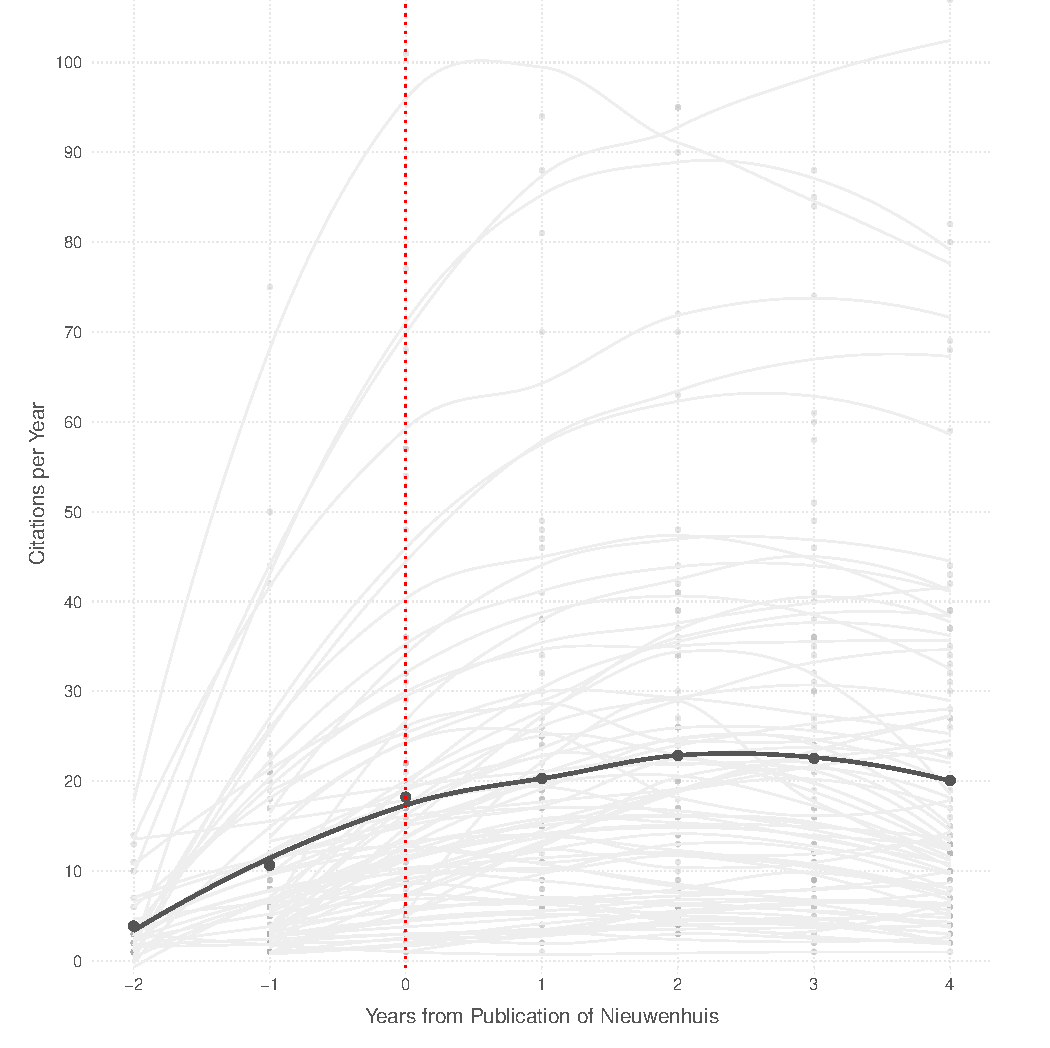
\includegraphics[scale=.7]{../figs/nw_growth_curve.pdf}
\caption{Number of Citations to Articles Containing the Error Per Year.}
\label{fig:niewenhuis}
\end{figure}

But citations to erroneous research do not need to decline after the error in the research is publicized. We only expect approving citations to decline. To estimate how many citations after the publication of Nieuwenhuis et al. are approving, we coded whether the citation was approving or not in 100 randomly chosen articles citing articles with the mistake (see SM \ref{approving_or_not} for details about the coding.) Of the 100, only one article noted concerns with the cited article, citing \cite{nieuwenhuis2011} for support. In all, there is strong evidence that approving citations are extremely common after the error is publicized.

We expected approving citations to articles making a statistical error to decline, but our expectations were tempered by the fact that publications about statistical errors do not gain the same publicity as retractions. To study how citations to retracted articles fare before, we leveraged a large novel dataset of retracted articles and citations to them. 

We used WoS to assemble the data. WoS indexes articles from over 9,500 natural science journals and 3,500 social science journals \cite{yong2013web}. (See Supplementary Materials (SM) \ref{web_of_science} for details about the WoS database.) To assemble the data, we searched WoS for retraction notices, used information in the retraction notice records to download retracted articles, and then downloaded citations to the retracted articles using WoS feature that allows you to access citations associated with an article. (For details about the method and robustness checks around data, see SM \ref{data_collection}.) 

Our final dataset has 3,029 retracted articles and 73,564 citations to the retracted articles. 65.2\% of the retracted articles are from Life Sciences and Biomedicine and 13\% are from Physical Sciences. (For a breakdown by field, see Table \ref{tab:ret_field}.) Data also show that the number of retractions has increased sharply over the last thirty years (see Fig. ~\ref{fig:n_retraction_notices_per_year}). Between 1989 and 1999, the number of retraction notices being published per year never crossed 20. Since then, there has been a sharp rise in the number of retraction notices per year. Between 2001, when 15 retraction notices were published, and 2015, the last year for which we have complete data, there was a near 30 fold increase when a total of 439 retraction notices were published. The pattern that we find is consistent with results from other studies looking at retraction rates \cite{steen2013has}.

The rapid rise in the number of retractions is likely a combination of increasing production and improvements in detection. But the bottom line is that there is an ever faster growing number of articles that the scientific community thinks should not have have been published in the first place. 

To understand why the articles are retracted, we coded a random sample of 100 retraction notices. Of the 100, 39\% mentioned plagiarism as one of the major reasons for retracting the article. (Plagiarism includes self-plagiarism, duplication of data, words, and publishing the same or similar article in multiple journals.) Major errors or fraud contributed to another 51\% of retractions, with fraud alone contributing to 24\% of retractions. Ethics violations (2) and conflict over authorship or approval from other authors (5) contributed to the rest. The percentage of retractions attributable to major errors or fraud in our data is similar to other research on reasons for retraction in other corpora. For instance, a study of 1,112 Biomedicine articles retracted between 1997 and 2009 found that 55\% were retracted for some type of misconduct \cite{budd2011retracted} (see also \cite{steen2010retractions}). All in all, articles are mostly retracted because the research cannot be trusted.

These flawed articles often accrue a fair number of citations before being retracted. In our data, the articles had been cited 39,792 times before being retracted. This is not unsurprising, given that it took, on average, 2.85 years for the article to be retracted. The median time before the article was retracted was two years (see Fig. \ref{fig:ttr}) with 28.1\% of the articles taking 4 or more years to be retracted. These numbers are similar to those obtained elsewhere. A study on time to retraction in the PubMed corpus found that the average time to retraction was approximately three years  \cite{steen2013has}. 

\begin{figure}[h]
\centering
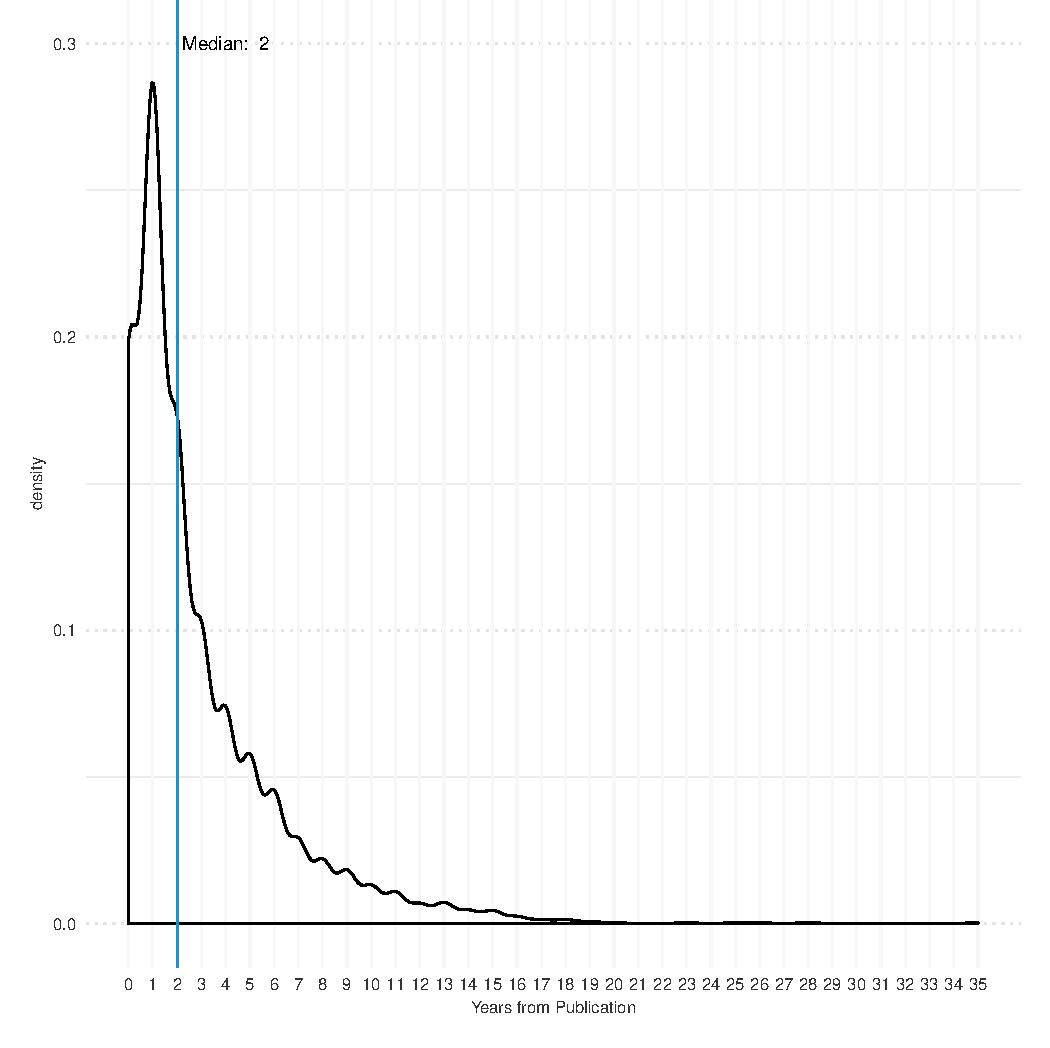
\includegraphics[scale=.7]{../figs/time_to_retraction.pdf}
\caption{Time to Retraction}
\label{fig:ttr}
\end{figure}

On the hunch that greater readership of more prominent journals would mean that problematic articles are flagged more quickly, we estimated the relationship between journal impact factor and average time to retraction. As Fig. \ref{fig:jif_ttr} shows, the relationship is flat---flawed articles in low ranked journals are retracted as quickly as flawed articles in higher ranked journals.

Given that a majority of retracted articles are retracted because of serious error or fraud, we expect retracted articles to \textit{never} be approvingly cited a year or more---taking account of long publication windows---after the retraction notice has been published. However, retracted articles were cited another 22,932 times between the year after they were retracted and August 2016. Thus, on average, the retracted articles received an additional 7.57 citations. Given the skew in retraction notices, with a bulk being published in recent years, these totals include very little post retraction data for many of the articles. In other words, the results are a \textit{lower bound} of the percentage of citations that happen after an article has been retracted.

To explore the frequency of citation before and after retracted, we plotted line graphs of total citations per article per year against year from the publication of retraction notice (see Fig. \ref{fig:pre_post_retraction}). And we overlaid the lines with the median number of citations per article per year. We limit ourselves to 10 years before and after the publication of retraction notice as the data are very sparse beyond that. The number of citations decline when the retraction notice is published (the median goes from 3 to 2 between the year retraction notice is published after next year) but is followed by a plateauing. Regressions that control for a time trend show the same (see Table \ref{tab:tab2}). Citations continue to accrue at a steady low rate long after the article has been retracted.

\begin{figure}[h]
\centering
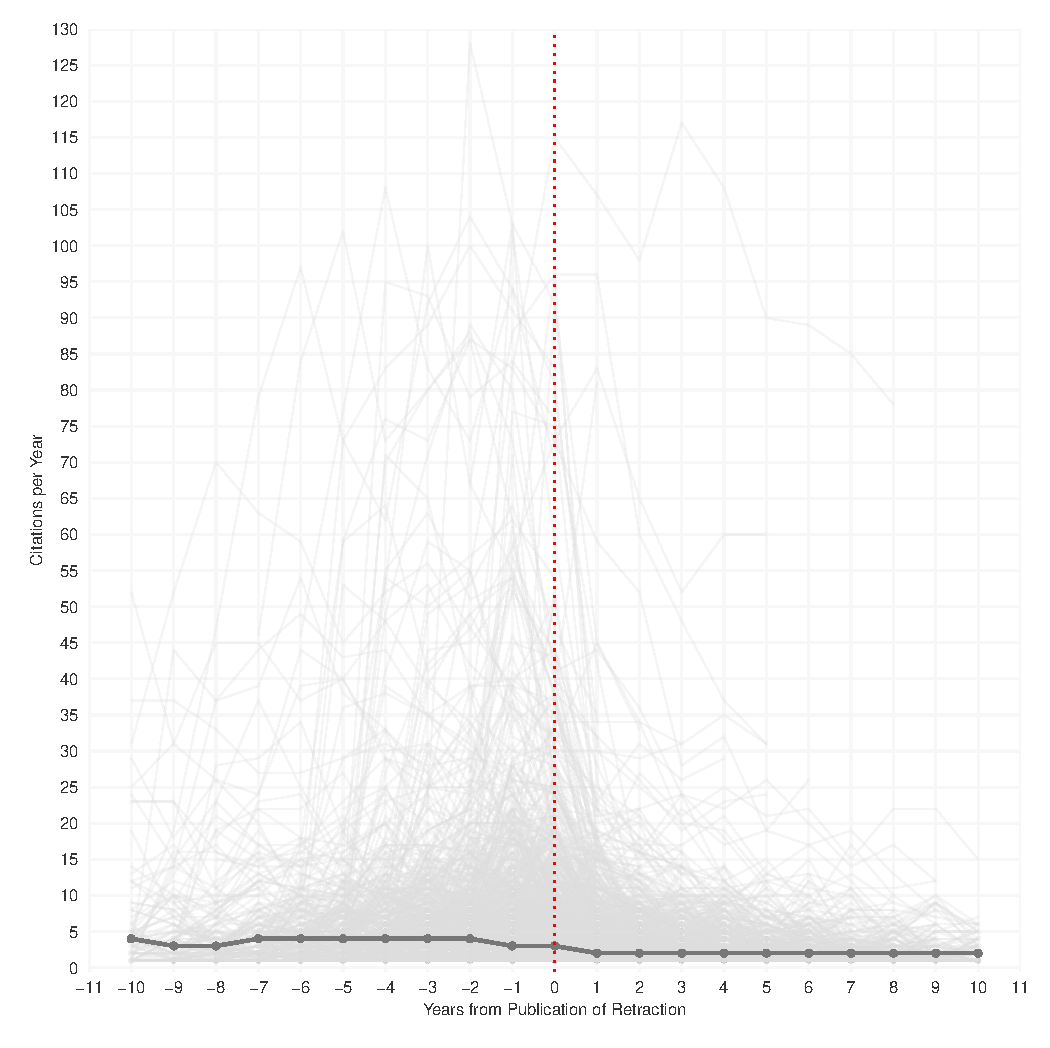
\includegraphics[scale=.7]{../figs/retracted_growth_curve.pdf}
\caption{Number of Citations to Retracted Articles per Year}
\label{fig:pre_post_retraction}
\end{figure}

To estimate how many of the citations are \textit{approving}, we coded a random sample of 100 articles that cited a retracted article pre-retraction and 275 articles that cited retracted research a year or more after the publication of the retraction notice. 97.7\% of the articles cited retracted research approvingly before or in the same year as the retraction was published. The rate drops to 91.4\% for articles citing retracted articles a year or more after retraction. (Fig. \ref{fig:prop_approving_per_year} plots proportion of citations approving by year.) In all, data suggest that problematic research continues to be approvingly cited at a high rate long after problems have been publicized.

\begin{figure}[t]
\centering
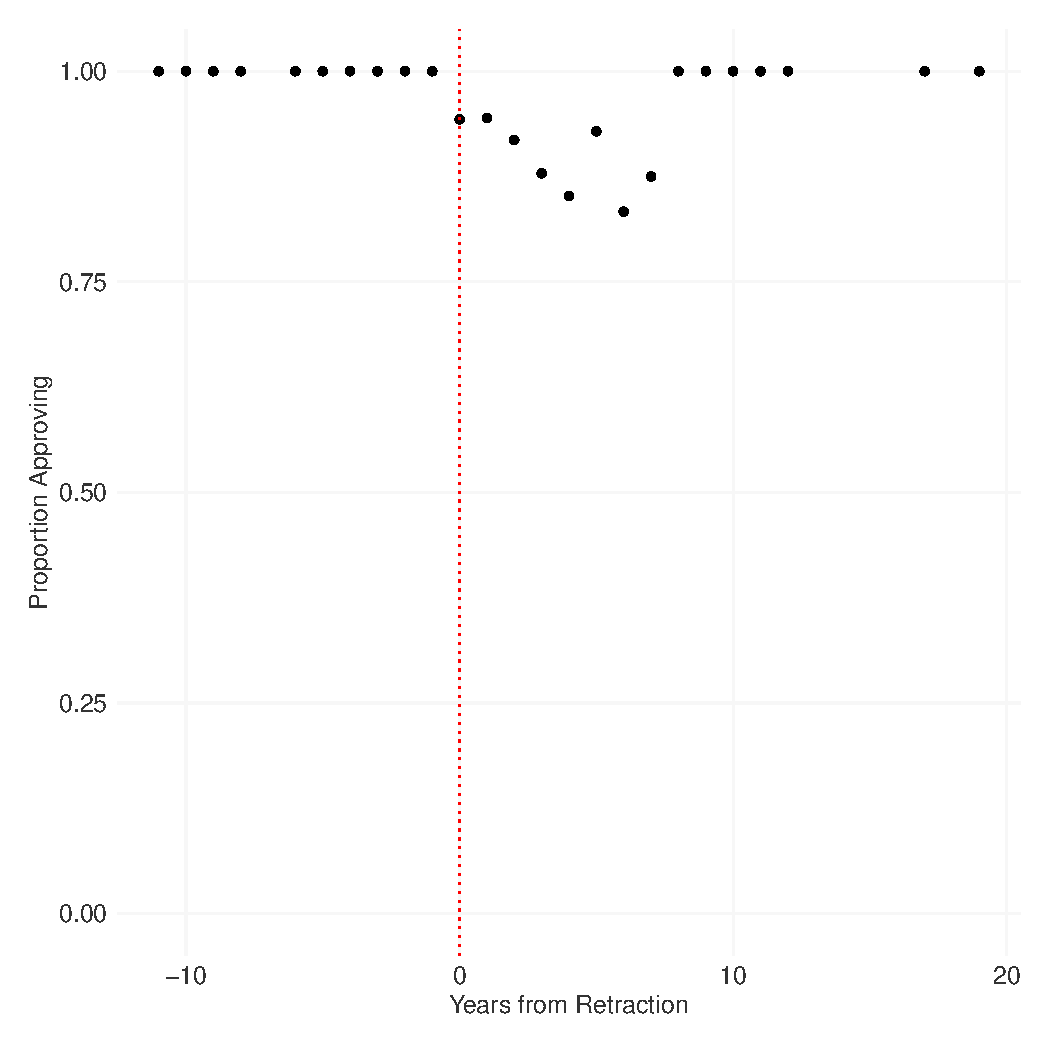
\includegraphics[width=10cm]{../figs/pre_post_prop_approving.pdf}
\caption{Proportion of Citations That Are Approving Per Year}
\label{fig:prop_approving_per_year}
\end{figure}

But why do researchers approvingly cite problematic research even after the problems have been publicized? It is likely because they are unaware of the problems. That is not the same as saying that they couldn't have known, but that there are still barriers to finding out. For instance, Google Scholar does not flag if an article has been retracted. Similarly, bibliographic software does not alert researchers that problems have been discovered about a paper in their bibliographic database \cite{davis2012persistence}. 

The cost of finding out is not zero but neither is it too high. Many academic publishers flag retracted articles with the prefix ``retracted.'' We think that the reason scientists do not mount the low barriers---spend time carefully vetting each article---is because serious pressures to publish leave them with little time and because they trust published research. 

There are two reasons why we think scientists trust published research. The first is that the rate of retractions isn extremely low. For instance, of the nearly 9.4 million articles published between 1950 and 2004 and available on PubMed, only 596 have been retracted \cite{cokol2007many}. In all likelihood, however, the true rate of serious errors in manuscripts is manifolds that rate. The same study estimates the rate at which articles ought to be retracted to be anywhere between 16.7 times to 167.8 times the actual rate. 

The other likely reason why scientists trust published research is that they believe that scientific misconduct is limited to a few people. And that optimism is likely driven by the fact that a few cases of fraud get a bulk of the attention, with reporting often focusing on personalities rather than processes. Cases like Diederik Stapel, who fabricated data behind at least 30 papers \cite{levelt2012flawed}, John Darsee, who faked data behind nearly 100 publications \cite{stewart1987integrity, anderson2013research, wallis1983fraud}, and Jan Hendrik Sch{\"o}n, who during a period in 2001 published a research paper every 8 days based on fabricated data \cite{service2003scientific, anderson2013research}, Andrew Wakefield, who published a paper linking MMR vaccine to autism using fabricated data \cite{wakefield1998retracted, deer2011case, godlee2011wakefield}, and Michael Lacour, who published a paper in \textit{Science} based on fabricated data \cite{broockman2015irregularities, mcnutt2015editorial} get a bulk of the attention (see also \cite{basu2006they, anderson2013research}).

But misconduct is not limited to a few bad actors. A large anonymous survey of early- and mid-career scientists found that nearly 2\% of the scientists reported fabricating, falsifying, or plagiarizing in the last \textit{three} years \cite{martinson2005scientists} (see also \cite{titus2008repairing}. Another study found that nearly 34\% of the respondents admitted to engaging in questionable research practices \cite{fanelli2009many}.

In all, researchers continue to approvingly cite problematic research because the search costs are relatively high. To ameliorate the issue, we need to build tools that provide information during the research discovery and production processes. For instance, a browser plug-in that highlights problematic articles listed on a web page is likely to be useful. Providing such a tool to editors at academic publishers can help ameliorate the problem.

\clearpage
\bibliographystyle{Science}

\begin{thebibliography}{10}

\bibitem{rubio2005spontaneous}
D.~Rubio, {\it et~al.\/}, {\it Cancer research\/} {\bf 65}, 3035 (2005).

\bibitem{torsvik2010spontaneous}
A.~Torsvik, {\it et~al.\/}, {\it Cancer research\/} {\bf 70}, 6393 (2010).

\bibitem{chang2013safety}
H.~Chang, {\it et~al.\/}, {\it Aesthetic plastic surgery\/} {\bf 37}, 802
  (2013).

\bibitem{kosaka2012therapeutic}
H.~Kosaka, {\it et~al.\/}, {\it Cancer gene therapy\/} {\bf 19}, 572 (2012).

\bibitem{paul2015comment}
H.~Y. Paul, B.~D. Haughom, E.~N. Hansen, {\it The Journal of arthroplasty\/}
  {\bf 30}, 718 (2015).

\bibitem{lin2013perioperative}
J.~Lin, L.~Zhang, H.~Yang, {\it The Journal of arthroplasty\/} {\bf 28}, 207
  (2013).

\bibitem{russo2017perioperative}
M.~W. Russo, N.~L. Parks, W.~G. Hamilton, {\it Orthopedic Clinics\/} {\bf 48},
  401 (2017).

\bibitem{kochan1992persistence}
C.~A. Kochan, J.~M. Budd, {\it Journal of the American Society for Information
  Science\/} {\bf 43}, 488 (1992).

\bibitem{budd1998phenomena}
J.~M. Budd, M.~Sievert, T.~R. Schultz, {\it JAMA\/} {\bf 280}, 296 (1998).

\bibitem{pfeifer1990continued}
M.~P. Pfeifer, G.~L. Snodgrass, {\it JAMA\/} {\bf 263}, 1420 (1990).

\bibitem{nieuwenhuis2011}
S.~Nieuwenhuis, B.~U. Forstmann, E.-J. Wagenmakers, {\it Nature neuroscience\/}
  {\bf 14}, 1105 (2011).

\bibitem{gelman2006}
A.~Gelman, H.~Stern, {\it The American Statistician\/} {\bf 60}, 328 (2006).

\bibitem{reuters2012web}
T.~Reuters  (2012).

\bibitem{yong2013web}
J.~Yong-Hak, {\it Thomson Reuters\/}  (2013).

\bibitem{steen2013has}
R.~G. Steen, A.~Casadevall, F.~C. Fang, {\it PLoS One\/} {\bf 8}, e68397
  (2013).

\bibitem{budd2011retracted}
J.~M. Budd, Z.~C. Coble, K.~M. Anderson, {\it Association of College and
  Research Libraries Conference\/} (2011), pp. 390--5.

\bibitem{steen2010retractions}
R.~G. Steen, {\it Journal of medical ethics\/} pp. jme--2010 (2010).

\bibitem{davis2012persistence}
P.~M. Davis, {\it Journal of the Medical Library Association\/} {\bf 100}, 184
  (2012).

\bibitem{cokol2007many}
M.~Cokol, I.~Iossifov, R.~Rodriguez-Esteban, A.~Rzhetsky, {\it EMBO reports\/}
  {\bf 8}, 422 (2007).

\bibitem{levelt2012flawed}
W.~J. Levelt, P.~Drenth, E.~Noort  (2012).

\bibitem{stewart1987integrity}
W.~W. Stewart, N.~Feder, {\it Nature\/} {\bf 325}, 207 (1987).

\bibitem{anderson2013research}
M.~S. Anderson, M.~A. Shaw, N.~H. Steneck, E.~Konkle, T.~Kamata, {\it Higher
  education: handbook of theory and research\/} (Springer, 2013), pp. 217--261.

\bibitem{wallis1983fraud}
C.~Wallis, {\it Time\/} {\bf 121}, 49 (1983).

\bibitem{service2003scientific}
R.~F. Service, {\it Science (New York, NY)\/} {\bf 299}, 31 (2003).

\bibitem{wakefield1998retracted}
A.~J. Wakefield, {\it et~al.\/}, {\it The Lancet\/} {\bf 351}, 637 (1998).

\bibitem{deer2011case}
B.~Deer, {\it BMJ\/} {\bf 342}, c5347 (2011).

\bibitem{godlee2011wakefield}
F.~Godlee, J.~Smith, H.~Marcovitch, {\it BMJ\/} {\bf 342}, c7452 (2011).

\bibitem{broockman2015irregularities}
D.~Broockman, J.~Kalla, P.~Aronow, {\it Work. pap., Stanford Univ.
  http://stanford. edu/~ dbroock/broockman\_kalla\_aronow\_lg\_irregularities.
  pdf\/}  (2015).

\bibitem{mcnutt2015editorial}
M.~McNutt, {\it Science\/} p. aaa6638 (2015).

\bibitem{basu2006they}
P.~Basu, {\it Nature medicine\/} {\bf 12}, 492 (2006).

\bibitem{martinson2005scientists}
B.~C. Martinson, M.~S. Anderson, R.~De~Vries, {\it Nature\/} {\bf 435}, 737
  (2005).

\bibitem{titus2008repairing}
S.~L. Titus, J.~A. Wells, L.~J. Rhoades, {\it Nature\/} {\bf 453}, 980 (2008).

\bibitem{fanelli2009many}
D.~Fanelli, {\it PloS one\/} {\bf 4}, e5738 (2009).

\end{thebibliography}


\clearpage

\section*{Acknowledgments}
Data and replication code are available on GitHub at \href{http://github.com/recite/propagation\_of\_error}{http://github.com/recite/propagation\_of\_error}. Both authors contributed equally to all aspects of the research. No funding was required for this article. The authors declare no conflicts of interest. We are grateful to Danielle Portnoy and Xiaoran Huang for assisting us with research, and to Andrew Gelman, Kabir Khanna, and Daniel Stone for offering valuable comments.

%Here you should list the contents of your Supplementary Materials -- below is an example. 
%You should include a list of Supplementary figures, Tables, and any references that appear only in the SM. 
%Note that the reference numbering continues from the main text to the SM.
% In the example below, Refs. 4-10 were cited only in the SM.

\clearpage

\appendix
\renewcommand\thesection{\arabic{section}}
\renewcommand\thetable{S\arabic{table}}  
\renewcommand\thefigure{S\arabic{figure}}
\setcounter{figure}{0}
\setcounter{section}{0}
\setcounter{table}{0}

\section*{Supplementary Materials}

\textbf{This PDF file includes:}
\begin{itemize}
\item Materials and Methods
\item Supplementary Text
\item Fig. S1-S4
\item Tables S1-S4
\end{itemize}

\section{Materials and Methods}

\subsection{Web of Science Indices}
\label{web_of_science}
WoS indexes articles from over 12,000 international journals and 148,000 conferences \cite{yong2013web}. WoS contains key citation indices including the \textit{Science Citation Index Expanded} (over 9,500 journals; 1900--present), \textit{Social Sciences Citation Index} (over 3,500 journals; 1900--present), \textit{Arts \& Humanities Citation Index} (over 1,700 journals; 1975--present), \textit{Conference Proceedings Citation Index} (over 170,000 conferences; 1990-present), \textit{Book Citation Index} (over 30,000 titles; 2005--present), among others. For a full list of titles included in the \textit{Science Citation Index Expanded}, \textit{Social Sciences Citation Index}, \textit{Arts \& Humanities Citation Index}, and \textit{Conference Proceedings Citation Index}, and a synopsis of the \textit{Book Citation Index}, see \url{https://github.com/recite/propagation\_of\_error/data/11\_wos/what\_is\_in\_wos/}.

\subsection{Steps for Creating the Retractions Dataset}
\label{data_collection}
To build a database of retracted articles, we started by creating a list of retraction notices. To do that, in August 2016, we searched WoS for titles containing the phrase ``retraction of.'' The search yielded more than 14,000 records. Using the ``corrections'' filter in WoS---it is a WoS flag for retraction and correction notices---we filtered the list to 4,085 retraction notices.

Next, we wrote software to automatically search the WoS database for retracted articles using the information in the retraction notice records. Retraction notice records did not contain consistent titles to allow us to a simple search. But 99\% of the retraction notices contained the year the original article was published, and 96\% listed the authors of the original work. We used these two pieces of information along with the name of the publication to search the WoS for the original articles. The search resulted in a list of 3,776 articles. We could not locate the remaining 309 retracted articles.

Due to the variability in the information contained in the retraction notice records, the automated search process returned the wrong article in some cases. Our aim was to have zero false positives even at the risk of some false negatives. With that aim, we created rules to flag potential false positives. First, if the list of authors of the retracted article did not match the list of authors for the relevant retraction notice record, we flagged the record as a potential false positive. Second, if the title of the retracted article did not contain the words ``retracted'' or ``retraction,'' we flagged it as a potential false positive. (It is standard practice for titles of original articles to be revised to indicate that the article has been retracted.) Third, we parsed the title of the retracted notices to extract the title of the original retracted article. And we flagged articles where the titles did not match as potential false positives. We then reviewed the potential false positives, filtering out all records where we could not verify the match. This resulted in a set of 3,084 articles. Finally, we checked for duplicates. We found 55. This left us with 3,029 articles. And that served as our final sample. 

As an additional robustness check, we manually checked a random sample of 100 retracted articles to confirm that the article had indeed been retracted. We found that all of them were.

To get a list of citations to these articles, we used the WoS functionality that allows users to access the list of citations to articles. We wrote software to automatically download citation records for each of the retracted articles. In total, we found 73,564 citations.

\subsection{Classifying Citations as Post-Retraction or Not}
A few retraction notices, retracted articles, and articles citing the retracted articles have earlier online (or conference) publication dates than the print publication dates recorded by WoS. As a result, post-retraction citations can be classified as otherwise. Or vice versa. To determine the impact of this issue and issues like these on our estimate of the lower bound of the proportion of citations that are made a year or more after the publication of the retraction notice, we manually recorded the online publication dates for a random sample of 300 citations to retracted articles, the associated retraction notices, and retracted articles. We could not retrieve 20 articles citing a retracted article.  Of the remaining 280 records, switching to online publication dates suggests that three articles were misclassified as post-retraction (2.2\%) and four were misclassified as not post-retraction (3.2\%). Taking these error rates at their face value, we re-calibrated our results. The recalibration results in an increase in the number of post-retraction citations, from 22,932 to 23,289. Or, the lower bound of the proportion of citations that happen the year after the retraction notice is published goes from 31.2\% to 31.7\%.

\subsection{Retracted Articles by Field}
\label{ret_art_by_field}
To understand the kinds of fields where retractions are more common, we used an augmented Web of Science research field categorization scheme to classify the articles. There is one caveat. Sometimes papers cover more than one topic. We just choose the first topic in these cases taking it to be the primary topic. 

As Table ~\ref{tab:ret_field} shows, 65\% of the retracted articles were published in the Life Sciences and Biomedicine field.  A distant second at 13\% is Physical Sciences, followed by Technology at 10.7\%. Social Sciences are at 5.5\%.  One reason why a large majority of the retractions are from the  Life Sciences and Biomedicine field may be simply because the field has more publications. But we cannot say anything definitely.

\subsection*{Coding Citations as Approving or Not}
\label{approving_or_not}
To estimate what proportion of the citations are approving, we coded a random sample. For Nieuwenhuis, we subset on citations to articles making the error after the publication of Nieuwenhuis, and then randomly chose a 100. For the retracted article dataset, we picked 375 citations using stratified random sampling so that we had 100 pre-retraction citations and 275 post-retraction citations. 

To code the citations, we downloaded the citing article. A research assistant then edited the citing article pdf to highlight where the retracted article was discussed in the citing article. The judgment of whether the article noted any concerns was made based on a review of the original retracted article pdf and the highlighted text. 

If an article does not note any concerns with the cited article, it implicitly \textit{approves} of the findings. Simply disagreeing with the conclusions of an article without noting any concern or citing the article in a he-said-she-said way still mean that the article is being cited in a way that suggests that its findings are trustworthy. So we code such instances as \textit{approving}. We code articles that note any concern with the citing article, even those unrelated to the cause of retraction, as \textit{disapproving}. 

We evaluated the reliability of the coding by having an independent rater code 50 randomly selected retracted articles. The two raters gave the same labels to all 50 articles. We take this as evidence that the coding was reliable.

In the Nieuwenhuis data, we could not locate one of the 100 articles, leaving us with 99 articles. Of the 99 articles, 2 were false positives---the articles did not cite erroneous research, but instead cited a paper with authors and title similar to published erroneous research. Of the 97 remaining articles, only one article noted concerns while citing an article making a mistake, citing Nieuwenhuis et al. \cite{nieuwenhuis2011} for support. 

In the retracted article data, we could not locate 32 articles, leaving us with 343 articles. There were no false positives. Of the 87 articles citing retracted articles before or in the same year the retraction notice was published, 85 (97.7\%) were approving. And of the 256 articles citing retracted articles the year after the retraction notice was published, 234 (91.4\%) were approving.

\section{Supplementary Text}

\subsection{Impact of Publication of Nieuwenhuis et al.}
In figure \ref{fig:niewenhuis}, we had plotted the total number of citations received per year by each of the papers making the mistake, the average number of citations received per year by articles making the mistake and smoothed \texttt{loess} growth curves in the manuscript. But the plot suggests that citation rates are skewed. To account for the skew, we switched means with medians (see Fig. ~\ref{fig:median_niewenhuis}). Doing so yields a similar pattern except for the expected intercept shift.

Nieuwenhuis et al. \cite{nieuwenhuis2011} flag articles where the error has potentially serious consequences for the results. So we subset on such articles and plot how the median number of citations varies across years. As Fig. \ref{fig:serious_niewenhuis} shows, the median number of citations steadily and modestly increase over time.

To more formally explore the change in citation rate as a consequence of the publication of \cite{nieuwenhuis2011}, we started with an `event study design' focusing on the citation rates to articles with the error. We regressed citations per year on a dummy for the year \cite{nieuwenhuis2011} was published, a linear time trend, and fixed effect for the article. We also cluster by articles to account for multiple observations per article. In effect, we are getting an average of within article changes after regressing out a linear time trend. Results show, if anything, a modest uptick in citations after \cite{nieuwenhuis2011} is published---a year after publication of \cite{nieuwenhuis2011}, articles containing the error get about four more citations per year compared to what they were getting before it (see Table \ref{tab:si_tab1}).

Our most complete analysis for the \cite{nieuwenhuis2011} data is a Difference-in-Differences (DID) analysis. DID gives us a better way to control for over time trends, though as you will see, the results echo the results from the simpler analysis. We estimated whether the difference in citation rates of articles making the error and those not making the error changed after the publication of \cite{nieuwenhuis2011}. In particular, we regressed citations per year on whether or not the article makes the error, the year(s) after the publication of \cite{nieuwenhuis2011}, and interaction between the two. We also include fixed effects for each article to do within article estimation. This allows us to circumvent concerns around skew in citations. And we again clustered the standard errors by article. 

Table \ref{tab:tab1} tabulates the results. Models (1), (3), and (5) define error as any article making the error. And Models (2), (4), and (6) refer to error as articles making ``potentially serious errors.'' As the table shows, 1 or 2 years after \cite{nieuwenhuis2011}, articles making the error were being cited more frequently vis-\`a-vis articles not making the error (Diff. $\sim$ 3). Three years out, we cannot still reject 0, suggesting that there is no evidence of a decline. For articles making ``potentially serious errors'', the story is much the same, except that the 1 and 2-year out estimates are closer to 3.5 additional citations per year than 3. And three years later, we still cannot say that the articles making ``potentially serious errors'' were being cited any less frequently.

\subsection{Number of Retracted Articles by Year in the WoS Dataset}
Fig. ~\ref{fig:n_retraction_notices_per_year} shows the number of retractions in the WoS dataset as a function of year of publication. As is clear, the number of retracted articles is increasing exponentially.

The rapid rise in the number of retractions is likely a combination of increasing production and improvements in detection. But the bottom line is that there is an ever faster growing number of articles which the scientific community thinks should not have have been published in the first place. As we show above, articles are not retracted for minor violations, they are mostly retracted for major lapses in the scientific process.

\subsection{Relationship Between Journal Impact Factor and Time to Retraction}
We estimated the relationship between journal impact factor and average time to retraction. Journals with higher impact factor have no shorter time to retraction than journals with lower impact factors (see Fig. \ref{fig:jif_ttr}).

\subsection{Rate of Citations Before And After Retraction}
Fig. \ref{fig:pre_post_retraction} elides over the fact that we do not observe data on all articles after all the plotted years after the publication notice. For instance, if the retraction notice was published in 2014, we only observe one more full year of citations---2015. Thus, to look more formally at the impact of publication of retraction notices a year, 2 years, and 3 years after, we create subsets of data where we have all the articles for which we have at least 1 year, 2 years, and 3 years worth of data after the publication of the retraction notice. To analyze these subsets, we use a pretty simple model. We regress the number of citations per year per article on years from retraction notice, a dummy for the cliff (1-, 2-, and 3- years after the publication of the retraction notice) and an interaction between the two. We cluster the standard errors by article to account for the fact that we have multiple observations per article. The results of the model can be seen in Table \ref{tab:tab2}.

As Table \ref{tab:tab2} shows, on average an article is cited about 5--6 times per year. But 1, 2, and three years later, an average article accrues about two less citations per year, a drop that is statistically and substantively significant. There is also a small negative slope in the number of citations per year for models that estimate the effect 1 and two years out. So the number of citations is slowly decreasing. But note that our priors are post-retraction, articles would not be cited. So we must compare the citation rate to 0. And there we can easily reject the 0---citation rate post publication of the retraction notice is not zero.  

\section{Tables S1 to S4}

% latex table generated in R 3.5.1 by xtable 1.8-2 package
% Sun Aug 05 19:57:13 2018
\begin{table}[!htb]
\centering
  \caption{Retraction Notices By Field}
\begin{tabular}{lrr}
  \hline
Field & Number of Notices & Percentage of Total \\ 
  \hline
Arts \& Humanities & 13 & 0.4 \\ 
  Life Sciences \& Biomedicine & 1974 & 65.2 \\ 
  Multidisciplinary & 157 & 5.2 \\ 
  Physical Sciences & 393 & 13.0 \\ 
  Social Sciences & 165 & 5.5 \\ 
  Technology & 325 & 10.7 \\ 
   \hline
\end{tabular}
\label{tab:ret_field}
\end{table}



% Table created by stargazer v.5.2.2 by Marek Hlavac, Harvard University. E-mail: hlavac at fas.harvard.edu
% Date and time: Fri, Aug 03, 2018 - 1:38:47 PM
% Requires LaTeX packages: dcolumn 
\begin{table}[!htbp] \centering 
  \caption{Change in the Number of Citations to Articles Containing the Error Per Year Before and After Publication of Nieuwenhuis} 
  \label{tab:si_tab1} 
\begin{tabular}{@{\extracolsep{5pt}}lD{.}{.}{-1} D{.}{.}{-1} } 
\\[-1.8ex]\hline 
\hline \\[-1.8ex] 
 & \multicolumn{2}{c}{\textit{Dependent variable:}} \\ 
\cline{2-3} 
\\[-1.8ex] & \multicolumn{2}{c}{Citations Per Year} \\ 
 & \multicolumn{1}{c}{All Articles with Mistakes} & \multicolumn{1}{c}{Articles with Potentially Serious Errors} \\ 
\\[-1.8ex] & \multicolumn{1}{c}{(1)} & \multicolumn{1}{c}{(2)}\\ 
\hline \\[-1.8ex] 
 Transition Date & 3.8^{**} & 5.0^{**} \\ 
  & (1.7) & (2.0) \\ 
  Time & 2.0^{***} & 2.1^{***} \\ 
  & (0.4) & (0.5) \\ 
  Constant & 12.4^{***} & 11.6^{***} \\ 
  & (1.9) & (2.1) \\ 
 \hline \\[-1.8ex] 
Observations & \multicolumn{1}{c}{487} & \multicolumn{1}{c}{276} \\ 
Akaike Inf. Crit. & \multicolumn{1}{c}{3,818.0} & \multicolumn{1}{c}{2,095.8} \\ 
Bayesian Inf. Crit. & \multicolumn{1}{c}{3,838.9} & \multicolumn{1}{c}{2,113.9} \\ 
\hline 
\hline \\[-1.8ex] 
\textit{Note:}  & \multicolumn{2}{r}{$^{*}$p$<$0.1; $^{**}$p$<$0.05; $^{***}$p$<$0.01} \\ 
\end{tabular} 
\end{table} 



% Table created by stargazer v.5.2.2 by Marek Hlavac, Harvard University. E-mail: hlavac at fas.harvard.edu
% Date and time: Fri, Aug 03, 2018 - 1:38:56 PM
% Requires LaTeX packages: dcolumn rotating 
\begin{sidewaystable}[!htbp] \centering 
  \caption{Difference-in-Difference Analysis of the Impact of Publication of Nieuwenhuis on the Number of Times per Year Articles Containing the Error Are Cited Vis-a-Vis Articles that Didn't Contain the Error} 
  \label{tab:tab1} 
\small 
\begin{tabular}{@{\extracolsep{5pt}}lD{.}{.}{-1} D{.}{.}{-1} D{.}{.}{-1} D{.}{.}{-1} D{.}{.}{-1} D{.}{.}{-1} } 
\\[-1.8ex]\hline 
\hline \\[-1.8ex] 
 & \multicolumn{6}{c}{\textit{Dependent variable:}} \\ 
\cline{2-7} 
\\[-1.8ex] & \multicolumn{6}{c}{Citations per year} \\ 
 & \multicolumn{2}{c}{1 year out} & \multicolumn{2}{c}{2 years out} & \multicolumn{2}{c}{3 years out} \\ 
\\[-1.8ex] & \multicolumn{1}{c}{(1)} & \multicolumn{1}{c}{(2)} & \multicolumn{1}{c}{(3)} & \multicolumn{1}{c}{(4)} & \multicolumn{1}{c}{(5)} & \multicolumn{1}{c}{(6)}\\ 
\hline \\[-1.8ex] 
 Treatment Date & 7.2^{***} & 7.7^{***} & 5.1^{***} & 5.5^{***} & 3.7^{***} & 3.9^{***} \\ 
  & (0.9) & (0.7) & (0.9) & (0.7) & (1.0) & (0.8) \\ 
  Error or Not & 1.5 & 0.004 & 2.1 & 0.6 & 2.8 & 1.6 \\ 
  & (2.5) & (2.8) & (2.4) & (2.7) & (2.4) & (2.6) \\ 
  Makes Error*Treatment Date & 3.1^{**} & 3.7^{***} & 2.7^{**} & 3.5^{***} & 1.7 & 2.1 \\ 
  & (1.2) & (1.3) & (1.2) & (1.3) & (1.3) & (1.5) \\ 
  Constant & 9.5^{***} & 10.2^{***} & 11.7^{***} & 12.6^{***} & 13.1^{***} & 14.0^{***} \\ 
  & (1.8) & (1.5) & (1.7) & (1.5) & (1.7) & (1.4) \\ 
 \hline \\[-1.8ex] 
Observations & \multicolumn{1}{c}{957} & \multicolumn{1}{c}{957} & \multicolumn{1}{c}{957} & \multicolumn{1}{c}{957} & \multicolumn{1}{c}{957} & \multicolumn{1}{c}{957} \\ 
Akaike Inf. Crit. & \multicolumn{1}{c}{7,328.2} & \multicolumn{1}{c}{7,327.8} & \multicolumn{1}{c}{7,408.8} & \multicolumn{1}{c}{7,407.5} & \multicolumn{1}{c}{7,474.9} & \multicolumn{1}{c}{7,475.2} \\ 
Bayesian Inf. Crit. & \multicolumn{1}{c}{7,357.4} & \multicolumn{1}{c}{7,357.0} & \multicolumn{1}{c}{7,437.9} & \multicolumn{1}{c}{7,436.7} & \multicolumn{1}{c}{7,504.0} & \multicolumn{1}{c}{7,504.4} \\ 
\hline 
\hline \\[-1.8ex] 
\textit{Note:}  & \multicolumn{6}{l}{$^{*}$p$<$0.1; $^{**}$p$<$0.05; $^{***}$p$<$0.01} \\ 
 & \multicolumn{6}{l}{Models (1), (3), and (5) define error as any article making the error.} \\ 
 & \multicolumn{6}{l}{And Models (2), (4), and (6) refer to error as articles making ``potentially serious errors.''} \\ 
\end{tabular} 
\end{sidewaystable} 



% Table created by stargazer v.5.2.2 by Marek Hlavac, Harvard University. E-mail: hlavac at fas.harvard.edu
% Date and time: Fri, Feb 05, 2021 - 9:49:48 AM
% Requires LaTeX packages: dcolumn 
\begin{table}[!htbp] \centering 
  \caption{Impact of Publication of Retraction Notice on the Number of Times Retracted Articles Are Cited per Year} 
  \label{tab:tab2} 
\begin{tabular}{@{\extracolsep{5pt}}lD{.}{.}{-1} D{.}{.}{-1} D{.}{.}{-1} } 
\\[-1.8ex]\hline 
\hline \\[-1.8ex] 
 & \multicolumn{3}{c}{\textit{Dependent variable:}} \\ 
\cline{2-4} 
\\[-1.8ex] & \multicolumn{3}{c}{Citations Per Year} \\ 
 & \multicolumn{1}{c}{1 Year Later} & \multicolumn{1}{c}{2 Years Later} & \multicolumn{1}{c}{3 Years Later} \\ 
\\[-1.8ex] & \multicolumn{1}{c}{(1)} & \multicolumn{1}{c}{(2)} & \multicolumn{1}{c}{(3)}\\ 
\hline \\[-1.8ex] 
 (1, 2, 3) Years After Notice & -2.4^{***} & -2.1^{***} & -1.9^{***} \\ 
  & (0.2) & (0.2) & (0.3) \\ 
  Years to Notice & -0.01 & -0.2^{***} & -0.3^{***} \\ 
  & (0.03) & (0.03) & (0.03) \\ 
  (1, 2, 3) Years After Notice*Years to Notice & -0.4^{***} & -0.2^{***} & 0.002 \\ 
  & (0.04) & (0.05) & (0.1) \\ 
  Constant & 6.0^{***} & 5.2^{***} & 4.7^{***} \\ 
  & (0.2) & (0.1) & (0.2) \\ 
 \hline \\[-1.8ex] 
Observations & \multicolumn{1}{c}{12,511} & \multicolumn{1}{c}{11,486} & \multicolumn{1}{c}{10,428} \\ 
Akaike Inf. Crit. & \multicolumn{1}{c}{83,835.6} & \multicolumn{1}{c}{76,511.3} & \multicolumn{1}{c}{69,534.9} \\ 
Bayesian Inf. Crit. & \multicolumn{1}{c}{83,880.2} & \multicolumn{1}{c}{76,555.4} & \multicolumn{1}{c}{69,578.4} \\ 
\hline 
\hline \\[-1.8ex] 
\textit{Note:}  & \multicolumn{3}{r}{$^{*}$p$<$0.1; $^{**}$p$<$0.05; $^{***}$p$<$0.01} \\ 
\end{tabular} 
\end{table} 


\section{Figures S1 to S4}

\begin{figure}[h]
\centering
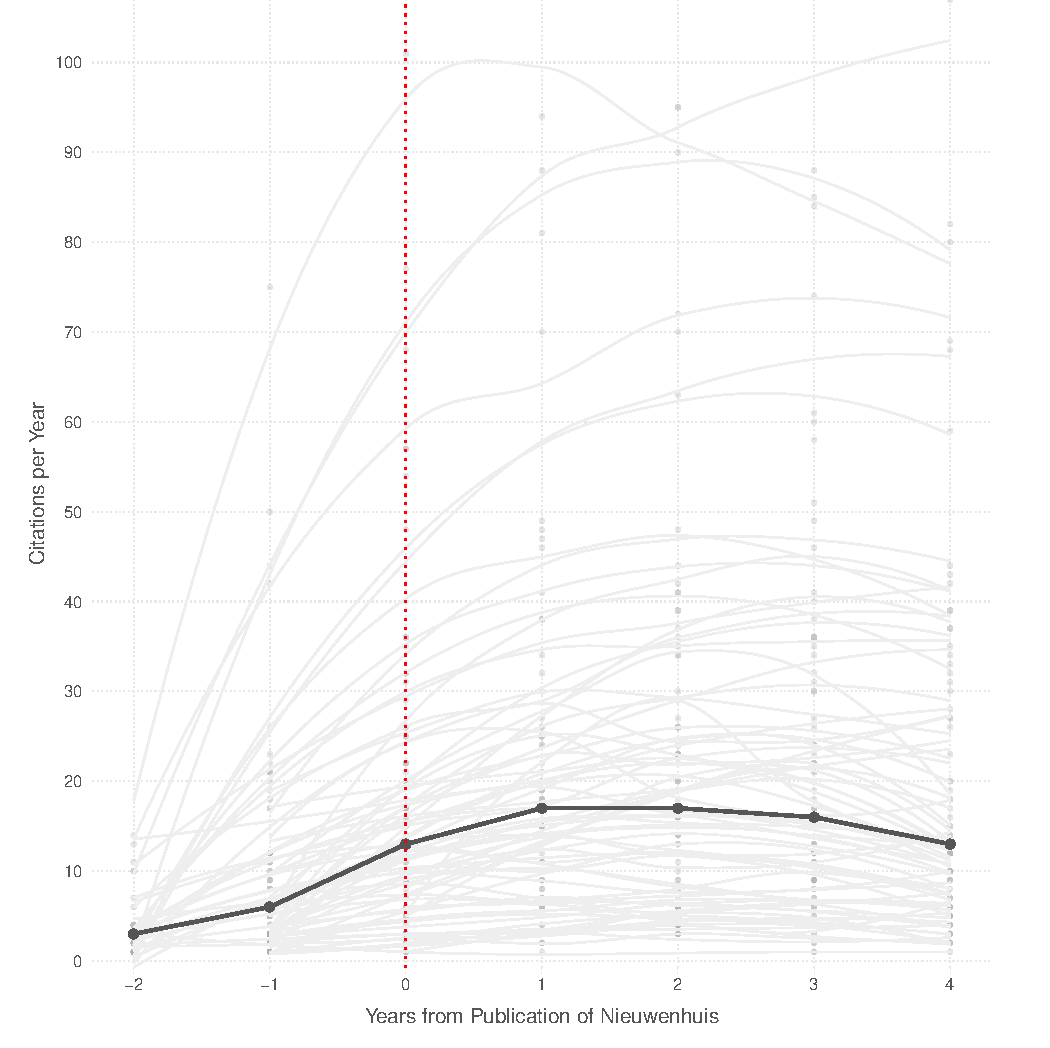
\includegraphics[scale=.7]{../figs/nw_median_growth_curve.pdf}
\caption{Total number of citations received per year by each of the papers making the mistake, and the median number of citations received per year by the articles.}
\label{fig:median_niewenhuis}
\end{figure}

\clearpage
\begin{figure}[h]
\centering
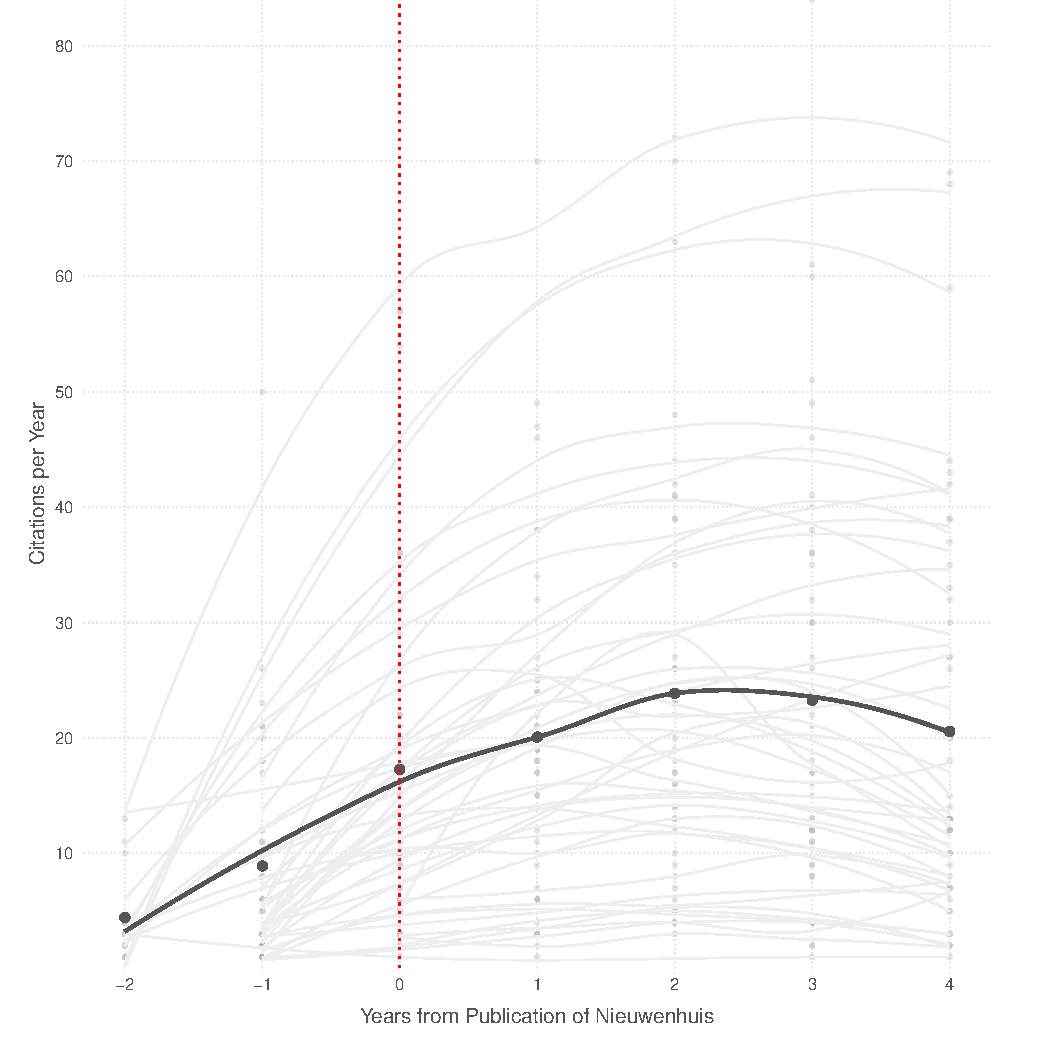
\includegraphics[scale=.7]{../figs/serious_nw_growth_curve.pdf}
\caption{Total number of citations received per year by articles making the mistake with `potentially serious' consequences for the results, and the average number of citations received per year by the articles.}
\label{fig:serious_niewenhuis}
\end{figure}

\begin{figure}[t]
\centering
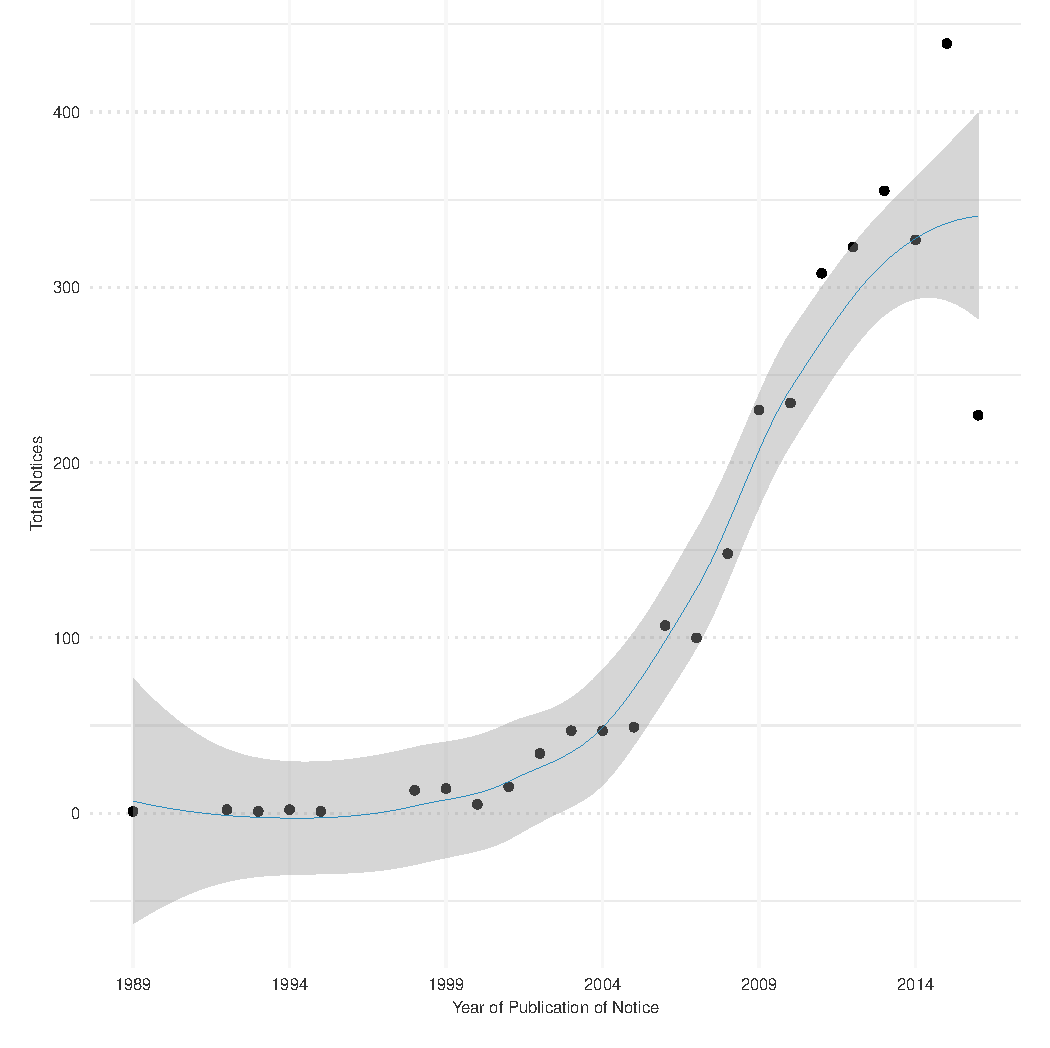
\includegraphics[scale=.7]{../figs/n_retraction_notices_by_year.pdf}
\caption{Retraction Notices Per Year}
\label{fig:n_retraction_notices_per_year}
\end{figure}

\begin{figure}[t]
\centering
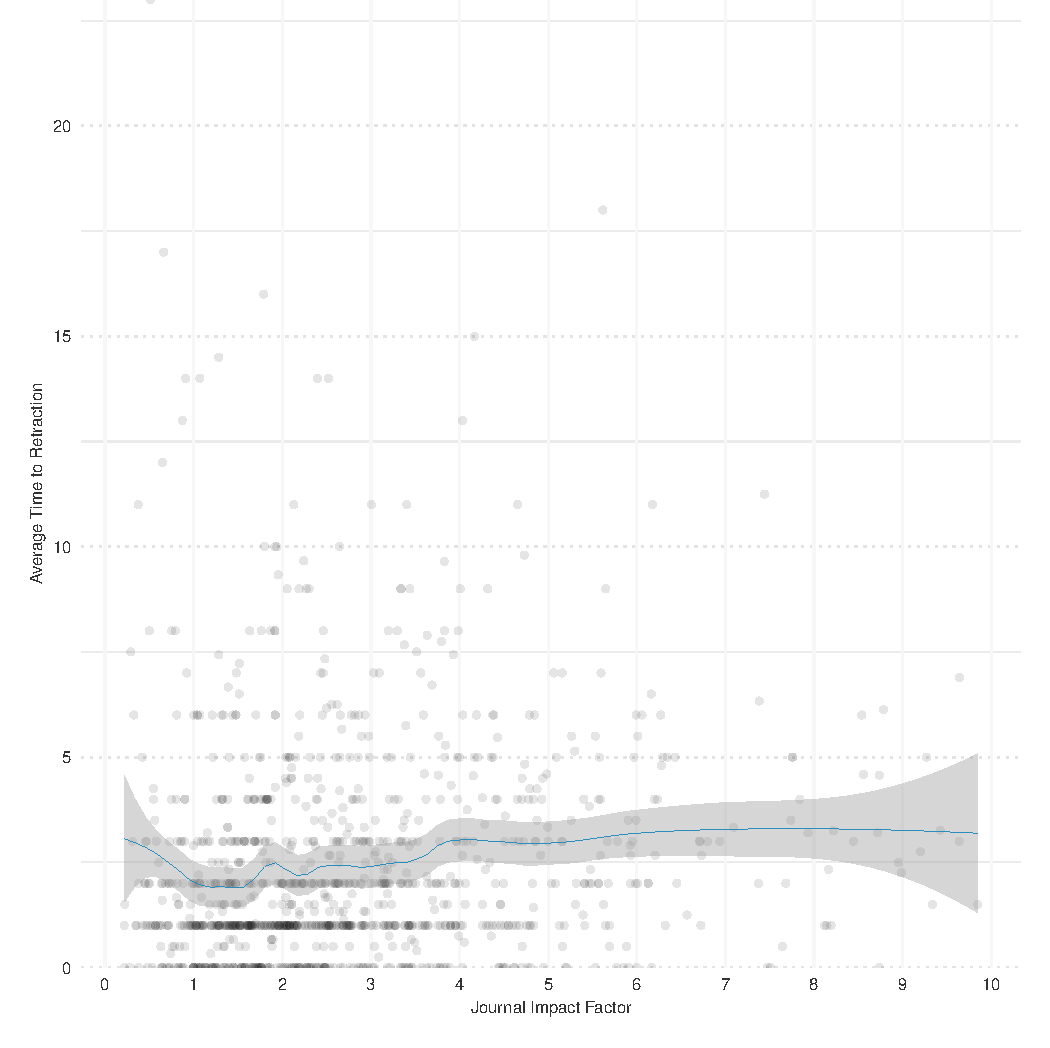
\includegraphics[scale=.7]{../figs/jif_time_to_retraction.pdf}
\caption{Relationship Between Journal Impact Factor and Time to Retraction}
\label{fig:jif_ttr}
\end{figure}


\end{document}
